\section{Theoretical Analysis}
\label{sec:analysis}

\begin{figure}[H] \centering
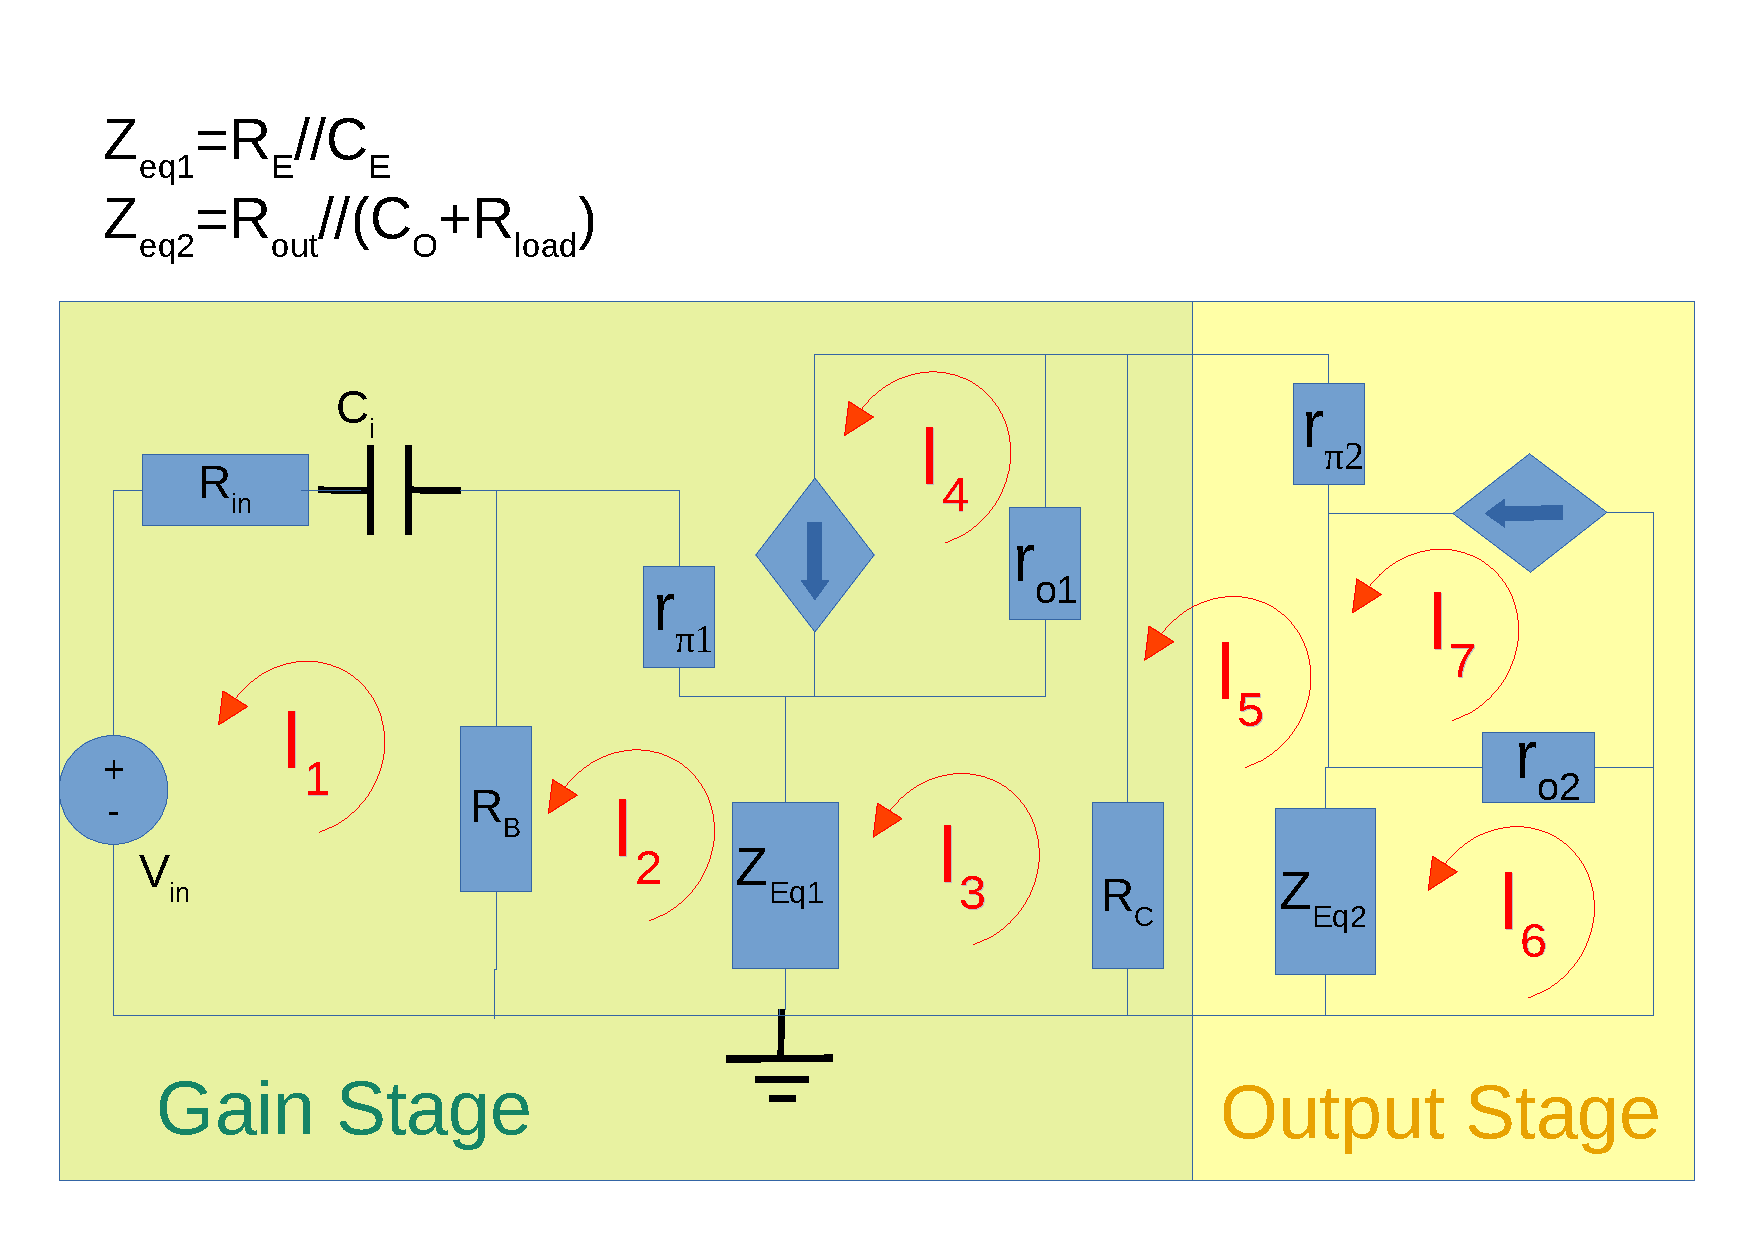
\includegraphics[width=0.7\linewidth]{../doc/circuit_freq.pdf}
\caption{Simplified circuit}
\label{fig:simp_cir}
\end{figure}

In this section for the incremental analysis part, we analyse the simplified circuit seen in the image above. When it reaches equilibrium, the capacitors work as a short circuit and that's what we will approximate them to.

\subsection{Gain Stage}
We start by analysing the circuit's operating point.
First we replace the bias circuit with a Thévenin equivalent resistance and voltage source given by:

\begin{equation}\label{eq:v_eq}
\begin{cases}
V_{eq}=\frac{R_{B2}}{R_{B1}+R_{B2}} V_{CC} \\
R_B=\frac{R_{B2}R_{B1}}{R_{B1}+R_{B2}}\\
\end{cases}
\end{equation}

Then we use mesh methods and the transistors relationships between currents to get the values of the circuit:

\begin{equation}\label{eq:Op1}
\begin{cases}
I_B=\frac{V_{eq}-V_{on}}{R_B+(1+\beta_f)R_{E}}\\
I_C=\beta_f I_B\\
I_E=(1+\beta_f)I_B\\
V_O=V_{CC}-R_C I_C\\
V_E=R_E I_E\\
V_{CE}=V_O-V_E\\
\end{cases}
\end{equation}

Now we need to solve the incremental circuit

\begin{equation}\label{eq:v1}
\begin{cases}
\frac{v_o}{v_i}=\frac{R_B}{R_B+R_S} R_C \frac{R_E-g_m r_\pi r_o}{(r_o+R_C+R_E)(R_{BS}+r_\pi+R_E)+g_m R_E r_o r_\pi - R_E^2}\\
R_{BS}=\frac{R_B R_S}{R_B+R_S}\\
\end{cases}
\end{equation}

Which can be approximated to:

\begin{equation}\label{eq:vs1}
\begin{cases}
\frac{v_o}{v_i}=-\frac{R_B}{R_B+R_S} \frac{g_m R_C}{1+g_m R_E}\\
\end{cases}
\end{equation}

 Using the mesh method on the gain circuit we get equations for the output and input impedances:
 
 \begin{equation}\label{eq:Z1}
\begin{cases}
Z_{I1}=\frac{1}{\frac{1}{R_B} \frac{r_{o1}+R_{C}+R_{E}}{(r_{o1}+R_{C}+R_{E})(r_{\pi 1}+R_{E})+g_{m1} R_{E} r_{o1} r_{\pi 1} - R_{E}^2}}\\
Z_{O1}= \frac{1}{\frac{1}{R_C} +\frac{\frac{1}{R_E}+\frac{1}{R_{\pi 1}+R_{BS}}}{r_{o1}(\frac{1}{R_E}+\frac{1}{R_{\pi 1}+R_{BS}}+\frac{1}{R_{o1}}+ \frac{g_{m1} r_{\pi 1}}{R_{\pi 1}+R_{BS}})}}\\
\end{cases}
\end{equation}

 Since we have capacitor $C_E$ in parallel with resisctor $R_E$, when charged we can consider it as a short circuit wich means $R_E=0$ in the equations above.
 \par
The values obtained for the output and input impedances and voltages is:

\begin{table}[H]
  \centering
  \begin{tabular}{|l|r|}
    \hline    
    {\bf Variable} & {\bf Value} \\ \hline
    \input{../mat/op1_tab.tex}
  \end{tabular}
  \caption{Gain stage values}
  \label{tab:sim1}
\end{table}

\subsection{Output stage}
We will consider that the input voltage in this stage is the output voltage of the gain stage. The reason we can make this approximation is explained at the end of this section.
\par
Just like in the last section we start by examine the circuit's operating point.  We use mesh analyses and current's relationships from the transistor's model again.

\begin{equation}\label{eq:Op2}
\begin{cases}
V_{I2}=V_O\\
I_{R_{out}}= \frac{V_{CC}-V_{EBON}-V_{I2}}{R_{out}}\\
V_{load}=V_{I2}+ V_{EBON}\\
\end{cases}
\end{equation}

Then again, we proceed for the incremental analyses

\begin{equation}\label{eq:v2}
\begin{cases}
\frac{v_{load}}{v_{i2}}=\frac{g_{m2}}{g_{m2}+g_{\pi 2}+g_{o2}+g_{out}}\\
Z_{I2}= \frac{g_{m2}+g_{\pi 2}+ g_{o2}+g_{out}}{g_{\pi 2} (g_{\pi 2}+ g_{o2}+g_{out})}\\
Z_{O2}= \frac{1}{g_{m2}+g_{\pi 2}+ g_{o2}+g_{out}}\\
\end{cases}
\end{equation}

The values obtained are:

\begin{table}[H]
  \centering
  \begin{tabular}{|l|r|}
    \hline    
    {\bf Variable} & {\bf Value} \\ \hline
    \input{../mat/op2_tab.tex}
  \end{tabular}
  \caption{Output stage values}
  \label{tab:sim1}
\end{table}


\subsection{Total circuit}
For this section we finally consider the circuit as a whole and join the two stages. Using the voltage divider law on a simple 1 voltage source and 2 resistors circuit we get:

\begin{equation}\label{eq:approx}
V_O=\frac{Z_O}{Z_O+Z_{eq}}V_I\\
\end{equation}

 Where O is the output, $V_I$ is the input voltage and $Z_{eq}$ is the other resistor. This means that if $Z_O >> Z_{eq}$ the input and output voltages are approximatelly the same. This means that if the output impedance of a stage is a lot lower than the next, $V_O\approx V_I$. We can consider the circuit as the combination of gain stage, output stage and load if $Z_{I2} >> Z_{O1}$ and $R_{load} >> Z_{O}$. So the total values' equations are:
 
\begin{equation}\label{eq:final}
\begin{cases}
\frac{v_{load}}{v_i}=\frac{g_B+\frac{g_{m2}}{g_{\pi 2}} g_B}{g_B+g_{out}+g_{o2}+\frac{g_{m2}}{g_{\pi 2}} g_B} \frac{v_o}{v_i}\\
V_{load}=V_{I2}+ V_{EBON}\\
Z_I=Z_{I1}\\
Z_O=\frac{1}{g_{o2}+\frac{g_{m2}}{g_{\pi 2}} g_B+g_{out}+g_B}\\
\end{cases}
\end{equation}

Where B is an equivalent resistance $R_B=r_{\pi 2} + Z_{O1}$
The values obtained for the final circuit are:

\begin{table}[H]
  \centering
  \begin{tabular}{|l|r|}
    \hline    
    {\bf Variable} & {\bf Value} \\ \hline
    \input{../mat/op3_tab.tex}
  \end{tabular}
  \caption{Total circuit values}
  \label{tab:sim1}
\end{table}

In the table below, we can see the node voltage in the operating point analysis

\begin{table}[H]
  \centering
  \begin{tabular}{|l|r|}
    \hline    
    {\bf Voltage} & {\bf Value (V)} \\ \hline
    \input{../mat/op4_tab.tex}
  \end{tabular}
  \caption{Operating Point Voltages}
  \label{tab:OP}
\end{table}

\subsection{Frequency response}
For the frequency response, we finally take into account the capacitors. Taking the circuit in \ref{fig:simp_cir} we use the mesh method to write the following system:

\begin{equation}\label{eq:freq}
\begin{cases}
I_1 (R_S+Z_{ci}+R_B) - I_2 R_B = v_{in}\\
-I_1 R_B +I_2 (R_B+r_{\pi 1} + Z_{eq1} -I_3 Z_{eq1} = 0\\
-I_2 Z_{eq1} + I_3 (Z_{eq1} + r_{o1} + R_C) -I_4 r_{o1} - I_5 R_C =0\\
I_2 r_{\pi 1} g_{m1} + I_4 = 0
-I_3 R_C + I_5 (r_{\pi 2} + R_C + Z_{eq2}) - I_6 Z{eq2} = 0\\
-I_5 Z_{eq2}+ I_6 (Z_{eq2} + r_{o2}) - I_7 r_{o2} =0\\
I_5 r_{\pi 2} g_{m2} +I_7 = 0\\
\end{cases}
\end{equation}

Solving this system for different frequencies, we get a graph of $gain(f)= \frac{(I_6 - I_5) Z_{eq2}}{v_{in}}$:

\begin{figure}[H] \centering
\includegraphics[width=0.7\linewidth]{../mat/tensao.pdf}
\caption{Frequency Response}
\label{fig:freq}
\end{figure}

Where we considered the approximation of the higher cutoff frequency to be in infinity.

%=========================================================================================================================


